\documentclass[
	11pt, % Default font size, select one of 10pt, 11pt or 12pt
	fleqn, % Left align equations
	a4paper, % Paper size, use either 'a4paper' for A4 size or 'letterpaper' for US letter size
	%oneside, % Uncomment for oneside mode, this doesn't start new chapters and parts on odd pages (adding an empty page if required), this mode is more suitable if the book is to be read on a screen instead of printed
]{LegrandOrangeBook}

% Book information for PDF metadata, remove/comment this block if not required 
\hypersetup{
	pdftitle={Title}, % Title field
	pdfauthor={Author}, % Author field
	pdfsubject={Subject}, % Subject field
	pdfkeywords={Keyword1, Keyword2, ...}, % Keywords
	pdfcreator={LaTeX}, % Content creator field
}

\definecolor{ocre}{RGB}{243, 102, 25} % Define the color used for highlighting throughout the book

\chapterimage{orange1.jpg} % Chapter heading image
\chapterspaceabove{6.5cm} % Default whitespace from the top of the page to the chapter title on chapter pages
\chapterspacebelow{6.75cm} % Default amount of vertical whitespace from the top margin to the start of the text on chapter pages

%----------------------------------------------------------------------------------------
\begin{document}
\section{Ley de Coulomb}
La ley de Coulomb establece de la fuerza \textit{F} entre dos cargas \textit{$Q_1$} y \textit{$Q_2$} son:
\begin{itemize}
\item A lo largo de la linea que los une.
\item Directamemte proporcional al producto \textit{$Q_1Q_2$} de las cargas.
\item Inversamente proporcional a la distancia \textit{R} que los separa
\end{itemize}
\begin{theorem}[Ley de Coulomb]
\begin{equation}
\label{eq:eqCoulomb}
F=\frac{kQ_1Q_2}{R^2}
\end{equation}
Donde:\\
\begin{itemize}
\item \textit{Q}: Cargas en Coulombs(C).
\item R: Distancia en metros(m).
\item F: Fuerza Newtons(N).
\end{itemize}
Constantes:
\begin{align*}
&\epsilon_0=8.854 \times 10^{-12}\simeq \frac{10^{-9}}{36\pi}F/m
&k=\frac{1}{4\pi\epsilon_0}\simeq 9\times 10^9 m/F
\end{align*}
\end{theorem}
%\begin{wrapfigure}{r}{0.5\textwidth}
%  \begin{center}
%    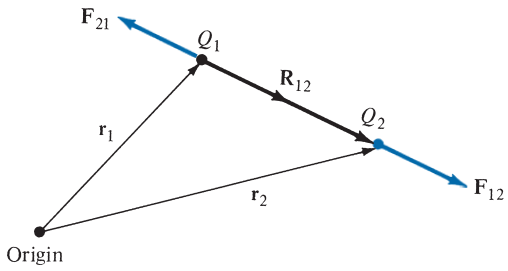
\includegraphics[width=0.48\textwidth]{CamposMag/CM10.png}
%  \end{center}
%  \caption{Birds}
%\end{wrapfigure}
Si las cargas $\textit{Q}_1$ y $\textit{Q}_2$ están localizadas en puntos cuyas posiciones están de forma vectorial $\textit{r}_1$ y $\textit{r}_2$(figura ), así la fuerza de $\textbf{F}_{12}$\footnote{Se lee: La fuerza de la carga 1 a la carga 2} sobre la carga 2 debido a la carga 1 esta dado por:
\begin{equation}
\boxed{F_{12}=\frac{Q_1Q_2}{4\pi\epsilon_0R^2}}
\end{equation}
\section{Intensidad de campo eléctrico}
La intensidad de campo eléctrico E es la fuerza que una unidad de carga positiva experimenta cuando se coloca en un campo eléctrico.
\begin{theorem}[Intensidad de campo eléctrico]
\begin{equation}
\label{eq:Intensidadcampoelectrico}
E=\frac{F}{Q}
\end{equation}
Donde:
\begin{itemize}
\item E: Intensidad de campo eléctrico(N/C) o Volts por metro(V/M).
\item F: Fuerza(N)
\item Q: Carga(Coulombs).
\end{itemize}
\end{theorem}
Para Q>0, la E esta en la misma dirección de la fuerza del F

\end{document}
